\documentclass[12pt,a4paper]{extreport}
\usepackage[a4paper, top=1.5cm, bottom=1.5cm, left=1.5cm, right=1.5cm]{geometry}
\setlength{\parindent}{1.25cm} % Отступ красной строки
\usepackage{listings} 
\usepackage{caption}

\usepackage{hyperref}
\usepackage{booktabs}
\usepackage{lipsum}

\usepackage{graphicx} % Для того, чтобы вставлять картинки.
\usepackage{wrapfig} % Картинка, обтекаемая текстом.
\usepackage{amssymb}
\usepackage{amsmath} % Чтобы вставлять обычный текст в формулу с помощью \text. Фигурная скобка в системе уравнений.

\usepackage{multicol} % Для написания текста в несколько колонок

\usepackage{setspace} % Для изменения межстрочного интервала внутри текста. \begin{spacing}{0.8}.

\usepackage{float}   % Чтобы была опция таблиц H, запрещающая им бегать по документу
\restylefloat{table}

\usepackage{gensymb} % Геометрические символы. (градусы \degree)..

\usepackage[warn]{mathtext} % Русские символы в формулах. Нужно писать до пакета babel. Указывает, что в формулах используются символы кириллицы, которые по умолчанию печатаются прямым шрифтом.

\usepackage[T2A]{fontenc} % Установить кодировку шрифта для отображения кириллицы в формулах.
\usepackage[utf8]{inputenc}

\usepackage[russian]{babel} % Для переноса текста. Нельзя указывать одновременно russian и english, так как использует язык, который стоит правее.

\usepackage{indentfirst} % Красная строка в первом абзаце.

\usepackage{comment} % Для многострочный комментариев.

\usepackage{subcaption}

\usepackage{colortbl} % Цветной текст.

%\DeclareSymbolFont{T2Aletters}{T2A}{cmr}{m}{it} % Сделать так, чтобы кириллица в формулах печаталась курсивом

\linespread{1.25} % Межстрочный интервал. По умолчанию 1.0

% Объявляем новую команду для переноса строки внутри ячейки таблицы
\newcommand{\specialcell}[2][c]{%
	\begin{tabular}[#1]{@{}c@{}}#2\end{tabular}}

\newcommand{\mA}{\; мА}
\newcommand{\uA}{\; мкА}
\newcommand{\uV}{\; мкВ}
\newcommand{\mm}{\; мм}
\newcommand{\m}{\; м}
\newcommand{\cm}{\; см}
\newcommand{\um}{\; мкм}
\newcommand{\dptr}{\; дптр}

\begin{document}
	
	\begin{center}
		\large
		\textsc{Лабораторная работа №4.5.1}
		
		\LARGE
		\textbf{Изучение гелий-неонового лазера}
		\\[5mm]

		\large
		Маслов Артём \\
		Казаков Данила \\
		Б01-104
		\\[3mm]
		18.03.2023
	\end{center}
			
	\section*{Аннотация}

В работе исследуется эффект Поккельса в кристалле необата лития. По интерференционной картине рассеянного света определяется двулучепреломление кристалла $n_o - n_e$. Полуволновое напряжение для данного образца определяется двумя способами. Первым способ -- по наблюдению периодических изменений интенсивности света на экране при увеличении постоянного напряжения на кристалле. Второй способ -- при подключении кристалла к источнику переменного напряжения, и наблюдению фигур Лиссажу при подключении первого входа осциллографа к источнику переменного напряжения, а второго к выходу фотодиода. По результатам измерений определяется коэффициент пропорциональности между внешним электрическим полем, приложенным к кристаллу, и разностью коэффициентов преломления.
	
	\section*{Теория}
Голография -- способ записи изображения, который позволяет по картине интенсивности восстановить полную информацию о волновом поле. Техника записи голограмм отображена на рис. 1. Важным свойством голограммы является возможность восстановить по её малому участку информацию обо всём объекте. 

\begin{figure}[tbp]	
	\centering
	\begin{minipage}{0.49\linewidth}
		\centering
		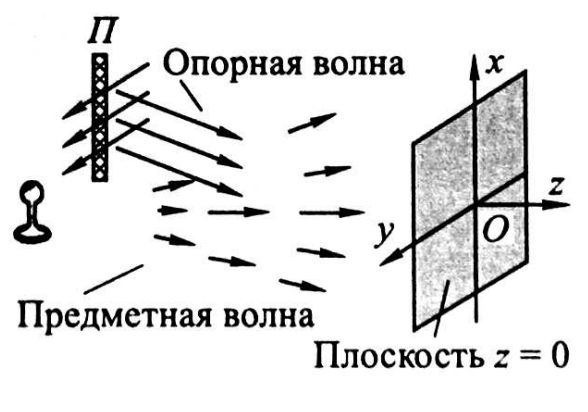
\includegraphics[width=0.8\linewidth]{../Изображения/Формирование.png}
		\caption{Запись голограммы}
	\end{minipage}
	\begin{minipage}{0.49\linewidth}
		\centering
		
\includegraphics[width=0.8\linewidth]{../Изображения/Габор.png}
		\caption{Зонная решётка Габора}
	\end{minipage}
\end{figure}

Назовём волну, падающую на предмет, предметной; а волну, падающую сразу на плёнку -- опорной. Эти волны должны быть когерентны. Тогда:
\begin{equation*}\label{key}
	t \propto a^2+a_о^2+2 a a_o \cos (\varphi - \varphi_о),
\end{equation*}
то есть сохраняется информация о фазе волны.

В частности, для точечного источника, считая, что $ f_п = a e^{i k z}  $ и $ f_о \approx a e^{i k r} $, получаем голограмму  с функцией пропускания
\begin{equation*}\label{key}
	t(x, y) \propto \left| a+ a e^{i k r}\right|^2.
\end{equation*}

Для обратного процесса -- восстановления -- применяют плоскую нормально падающую волну. Считая $ f_- (x, y) \equiv 1, $ на выходе голограммы точечного источника получим:
\begin{equation*}\label{key}
	f_+ (x, y) = \left| a+ a e^{i k r}\right|^2 = 2 a^2 (1+\cos (k r)) = 2 a^2 + a^2 e^{i k r} +a^2 e^{- i k r}.
\end{equation*}
Отсюда видна структура полученной волны: суперпозиция плоской и двух сферических волн (соответствующих действительному и мнимому источникам).

Голограмма точечного источника имеет вид колец (рис. \ref{fig:screenshot1}) с радиусами
\begin{equation*}\label{key}
	\rho_m = \sqrt{m \lambda z_0},
\end{equation*}
где нечётному $ m $ соответствуют тёмные кольца.

Одним из свойств голограммы является её разрешающая способность, определяемая выражением:
\begin{equation*}\label{key}
	\Delta x \sim \frac{\lambda}{D} z_0,
\end{equation*}
где $ z_0 $ -- расстояние от источника до его голограммы, а $ D $ -- размер голограммы.




	\section*{Описание экспериментальной установки}

Схема экспериментальной установки приведена на рисунке:

\begin{figure}[H]
	\centering
	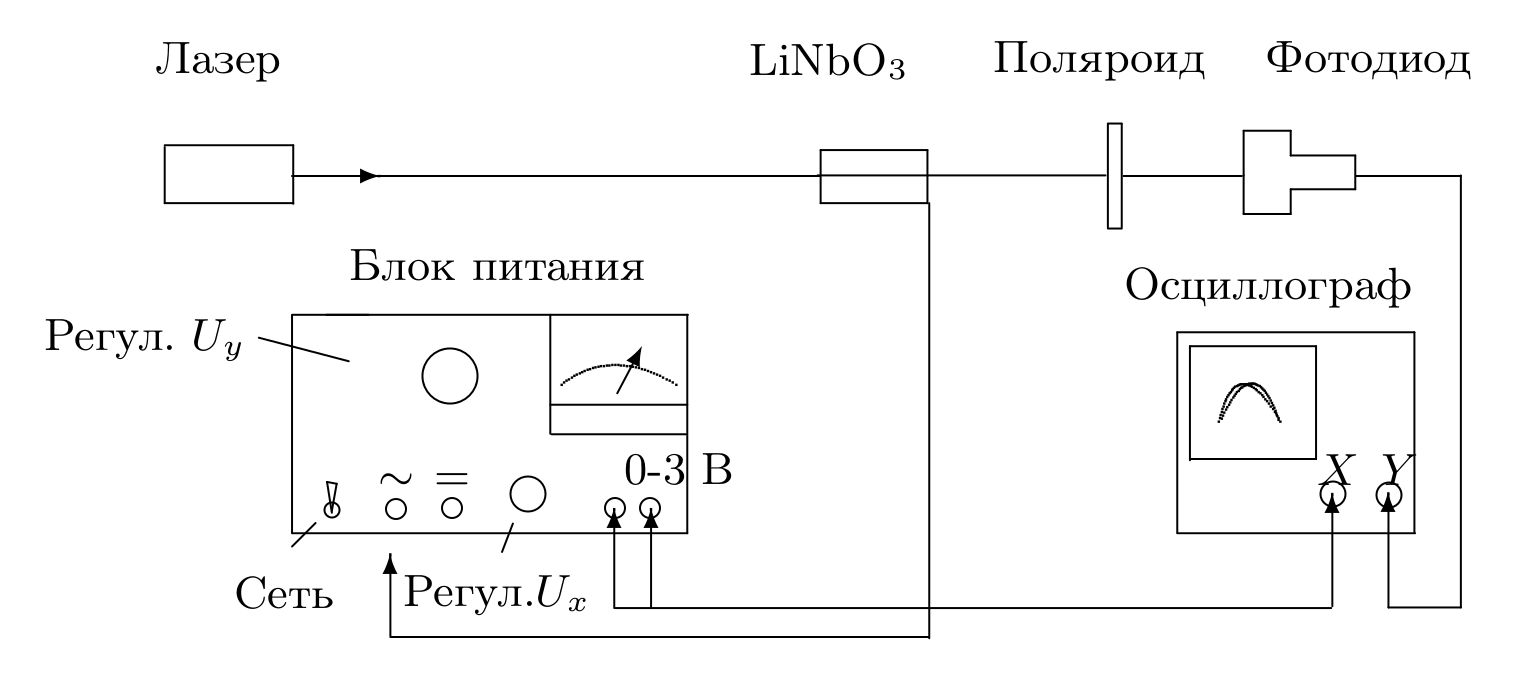
\includegraphics[width=0.8\textwidth]{../Изображения/facility.png}
	\caption{Схема экспериментальной установки}
\end{figure}

Луч света от лазера со встроенным вертикальным поляризатором попадает на кювету с кристаллом необата лития. Перед кюветой можно разместить матовую рассеивающую пластинку. Главная оптическая ось кристалла ориентирована вдоль направления распространения луча. После кюветы расположен поляроид. Результат интерференции наблюдается на экране. На кристалл можно подавать высоковольтное постоянное и переменное напряжение с помощью источника напряжения. Если подавать на кристалл переменное напряжение, то для исследования результата интерференции используется фотодиод, выход которого подключается к одному каналу осциллографа. Ко второму входу осциллографа подключается сигнал с источника напряжение.

	\section*{Оборудование}

\begin{enumerate}
	\item Оптическая скамья с набором рейтеров и осветителем.
	
	\item Зелёный светофильтр.
	
	\item Два поляроида.
	
	\item Чёрное зеркало.
	
	\item Полированная эбонитовая пластинка.
	
	\item Стопа стеклянных пластинок.
	
	\item Пластинки в 1/2, 1/4 и 1 длину волны для зелёного света.
\end{enumerate}
	
	\section*{Результаты измерений}

\begin{wrapfigure}{r}{0.3 \textwidth}
	\centering
	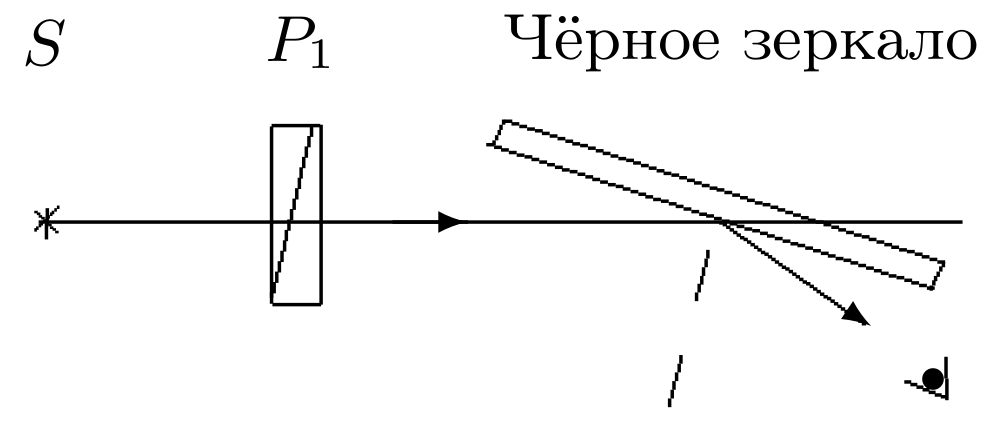
\includegraphics[width=0.28\textwidth]{../Изображения/black mirror.png}
\end{wrapfigure}

1. С помощью метода чёрного зеркала было определено разрешённое направление первого поляроида $\varphi_1 = 87^{\circ} \pm 1^{\circ}$. Поляроид пропускает свет, плоскость колебаний которого горизонтальная.

С помощью первого поляроида было определено разрешённое направление второго поляроида $\varphi_2 = 115^\circ \pm 1^{\circ}$. Поляроид пропускает свет, плоскость колебаний которого вертикальная.

2. Определим показатель преломления эбонита по формуле:
$$
n = \tg \varphi_Б
$$
Угол Брюстера без светофильтра $\varphi_{Б1} = 52^\circ \pm 3^\circ$. \\
Угол Брюстера со светофильтром $\varphi_{Б2} \in [46^\circ \pm 3^\circ; 54^\circ \pm 3^\circ]$.

$n_1 = 1,28 \pm 0,13$ \\
$n_2 \in [1,04 \pm 0,10; 1,38 \pm 0,14]$.

Погрешность косвенных измерений оценим по формуле:
$$
\sigma_n = \frac{\partial n}{\partial \varphi} \sigma_\varphi = \frac{\sigma_\varphi}{\cos^2 \varphi}
$$

Табличное значение показателя преломления эбонита $n_{табл} = 1,6 \div 1,7$.

Расхождение табличных и экспериментальных значений показателя преломления скорее всего связано с неточностью определения угла Брюстера, так как минимальная интенсивность определялась на глаз.

\begin{wrapfigure}{r}{0.3 \textwidth}
	\centering
	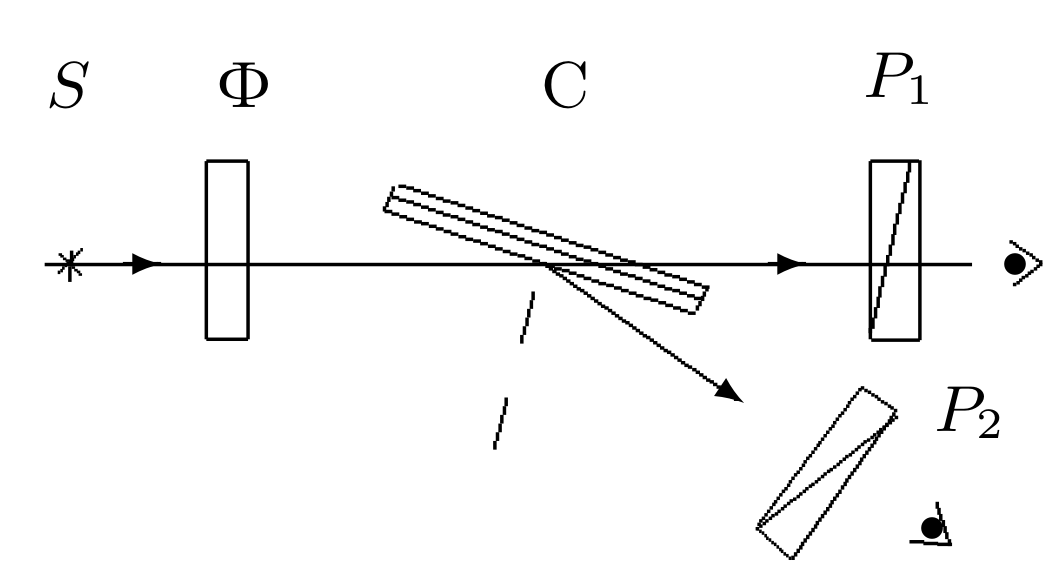
\includegraphics[width=0.28\textwidth]{../Изображения/glass stack.png}
\end{wrapfigure}

3. Исследуем поляризационные свойства стопы стеклянных пластин при падении неполяризованного света под углом Брюстера.

Для света, прошедшего стопу стеклянных пластин, интенсивность горизонтальной компоненты больше интенсивности вертикальной.

У света отражённого от стопы стеклянных пластин горизонтальная компонента практически отсутствует, а вертикальная компонента хорошо видна.

Интенсивность вертикальной компоненты отражённого от стопы стеклянных пластин света больше интенсивности вертикальной компоненты прошедшего света.

\begin{wrapfigure}{r}{0.3 \textwidth}
	\centering
	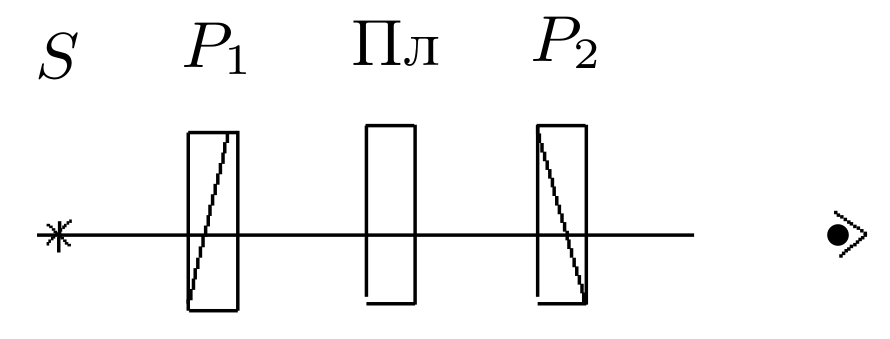
\includegraphics[width=0.28\textwidth]{../Изображения/main directions.png}
\end{wrapfigure}

4. Определим главные направления двоякопреломляющих пластин.

Пластина <<2 в кружочке>>. Направления наименьшей интенсивности: \\
$\varphi_{11} = 16^\circ$. \\
$\varphi_{12} = 110^\circ$. \\
$\varphi_{13} = 196^\circ$. \\
$\varphi_{14} = 288^\circ$. \\

Пластина <<2>>. \\
$\varphi_{11} = 40^\circ$. \\
$\varphi_{12} = 130^\circ$. \\
$\varphi_{13} = 220^\circ$. \\
$\varphi_{14} = 310^\circ$. \\

5. Добавим к схеме для определения главных направлений зелёный фильтр и повернём главные направления исследуемых пластин на $45^\circ$ вокруг главной оптической оси системы, оба поляроида установим в горизонтальное положение пропускания. Если исследуемая пластина $\frac{\lambda}{2}$, то сквозь систему свет проходить не будет.

В результате эксперимента определили, что пластина <<2>> -- пластина $\frac{\lambda}{2}$ -- на выходе создаёт линейную поляризацию, пластина <<2 в кружочке>> -- пластина $\frac{\lambda}{4}$ -- на выходе создаёт эллиптическую поляризацию.

6. С помощью пластинки чувствительного оттенка в $\lambda$ определили, что оси $\varphi_0 = 155^\circ$ соответствует большая скорость распространения, так как в этом случае проходящий систему свет приобретает голубую окраску. В перпендикулярном направлении окраска проходящего света -- оранжевая.

7. Исследуем интерференцию поляризованных лучей. Разместим между скрещенными поляроидами мозаичную слюдяную пластинку, собранную из 4 узких полосок слюды, лежащих по сторонам квадрата (две полоски $\frac{\lambda}{4}$, одна $\frac{\lambda}{2}$ и ещё одна $\frac{3\lambda}{4}$). В центре слюды нет, главные направления пластинок ориентированы параллельно сторонам квадрата.

Наблюдаемые картины при вращении поляроида $P1$ при неизменном $P2$.

\begin{figure}
	\centering
	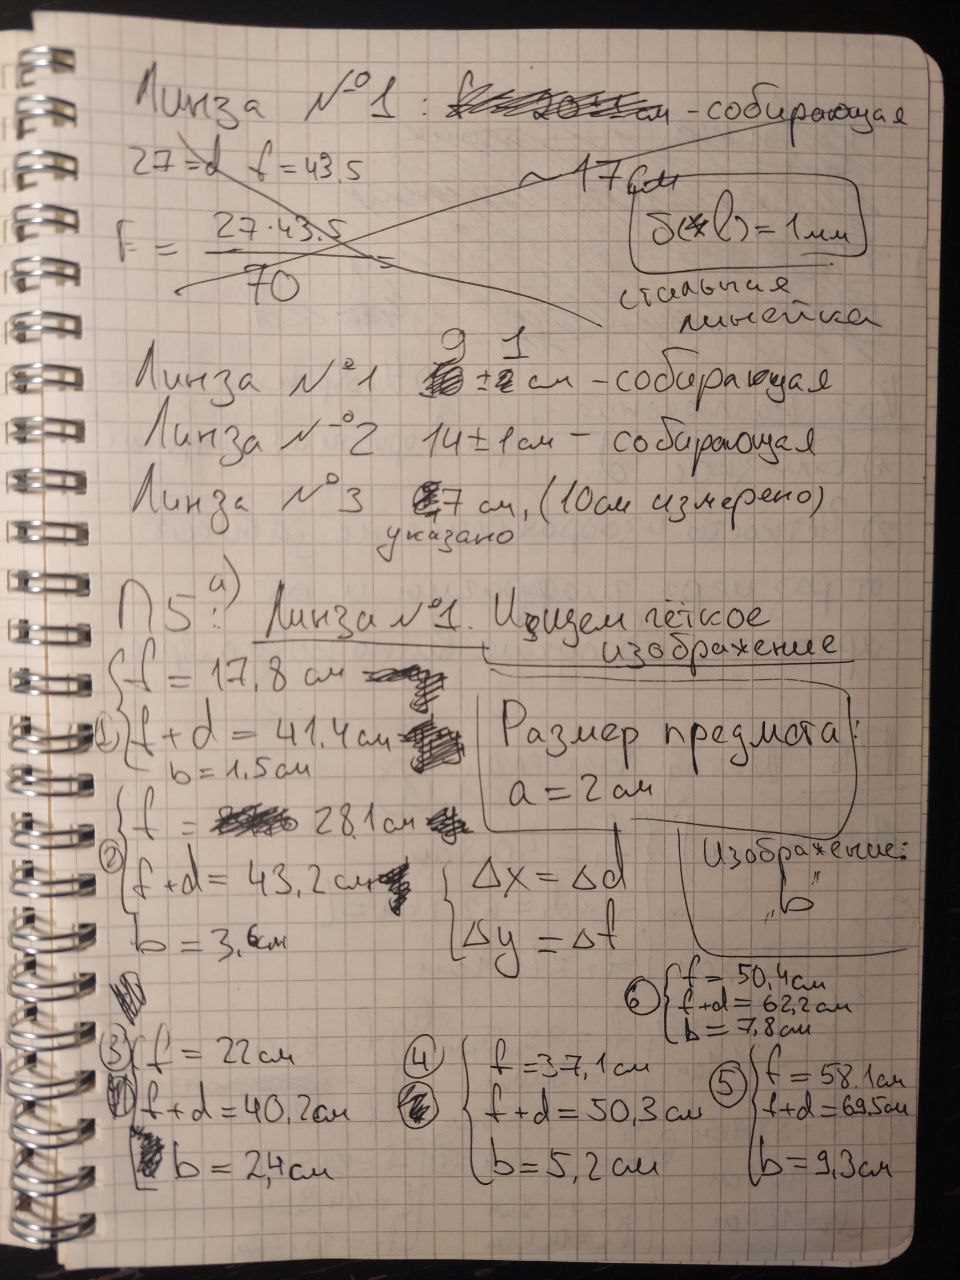
\includegraphics[width=0.3\textwidth]{../Изображения/1.jpg}
\end{figure}

\begin{figure}
	\centering
	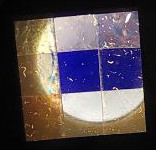
\includegraphics[width=0.3\textwidth]{../Изображения/2.jpg}
	\caption{На фотографии квадраты видны, как окрашены в синий, при наблюдении глаз воспринимал этот цвет как чёрный.}
\end{figure}

\begin{figure}
	\centering
	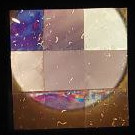
\includegraphics[width=0.3\textwidth]{../Изображения/3.jpg}
	\caption{На фотографии квадраты видны, как окрашены в синий, при наблюдении глаз воспринимал этот цвет как чёрный.}
\end{figure}

Наблюдаемые картины при вращении поляроида $P2$ при неизменном $P1$.

\begin{figure}
	\centering
	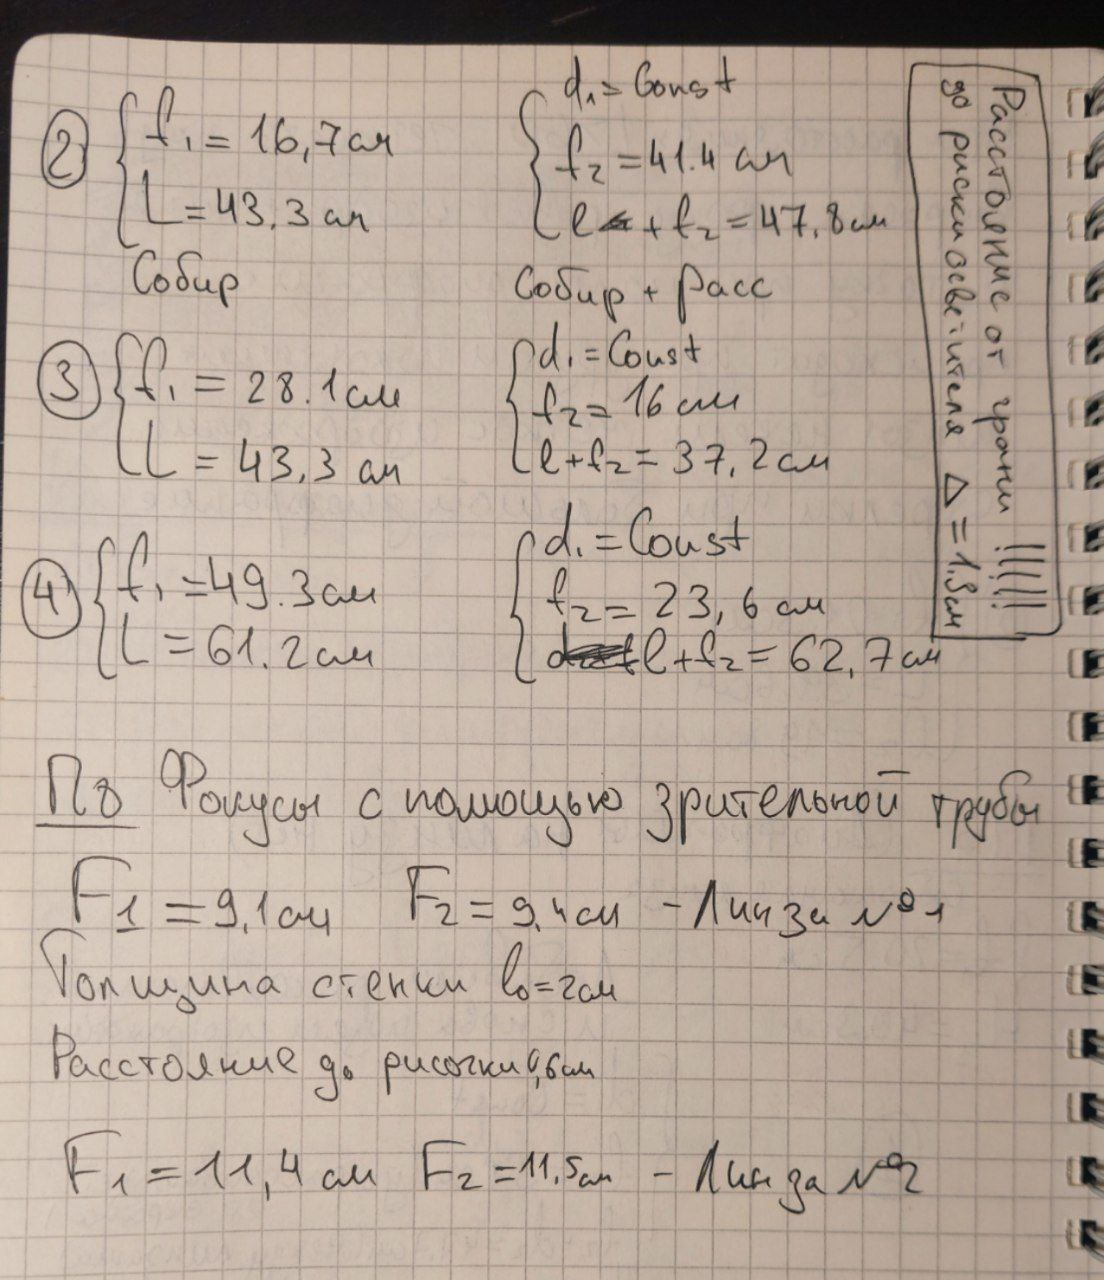
\includegraphics[width=0.3\textwidth]{../Изображения/4.jpg}
\end{figure}

\begin{figure}
	\centering
	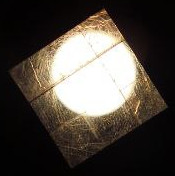
\includegraphics[width=0.3\textwidth]{../Изображения/5.jpg}
\end{figure}

\begin{figure}
	\centering
	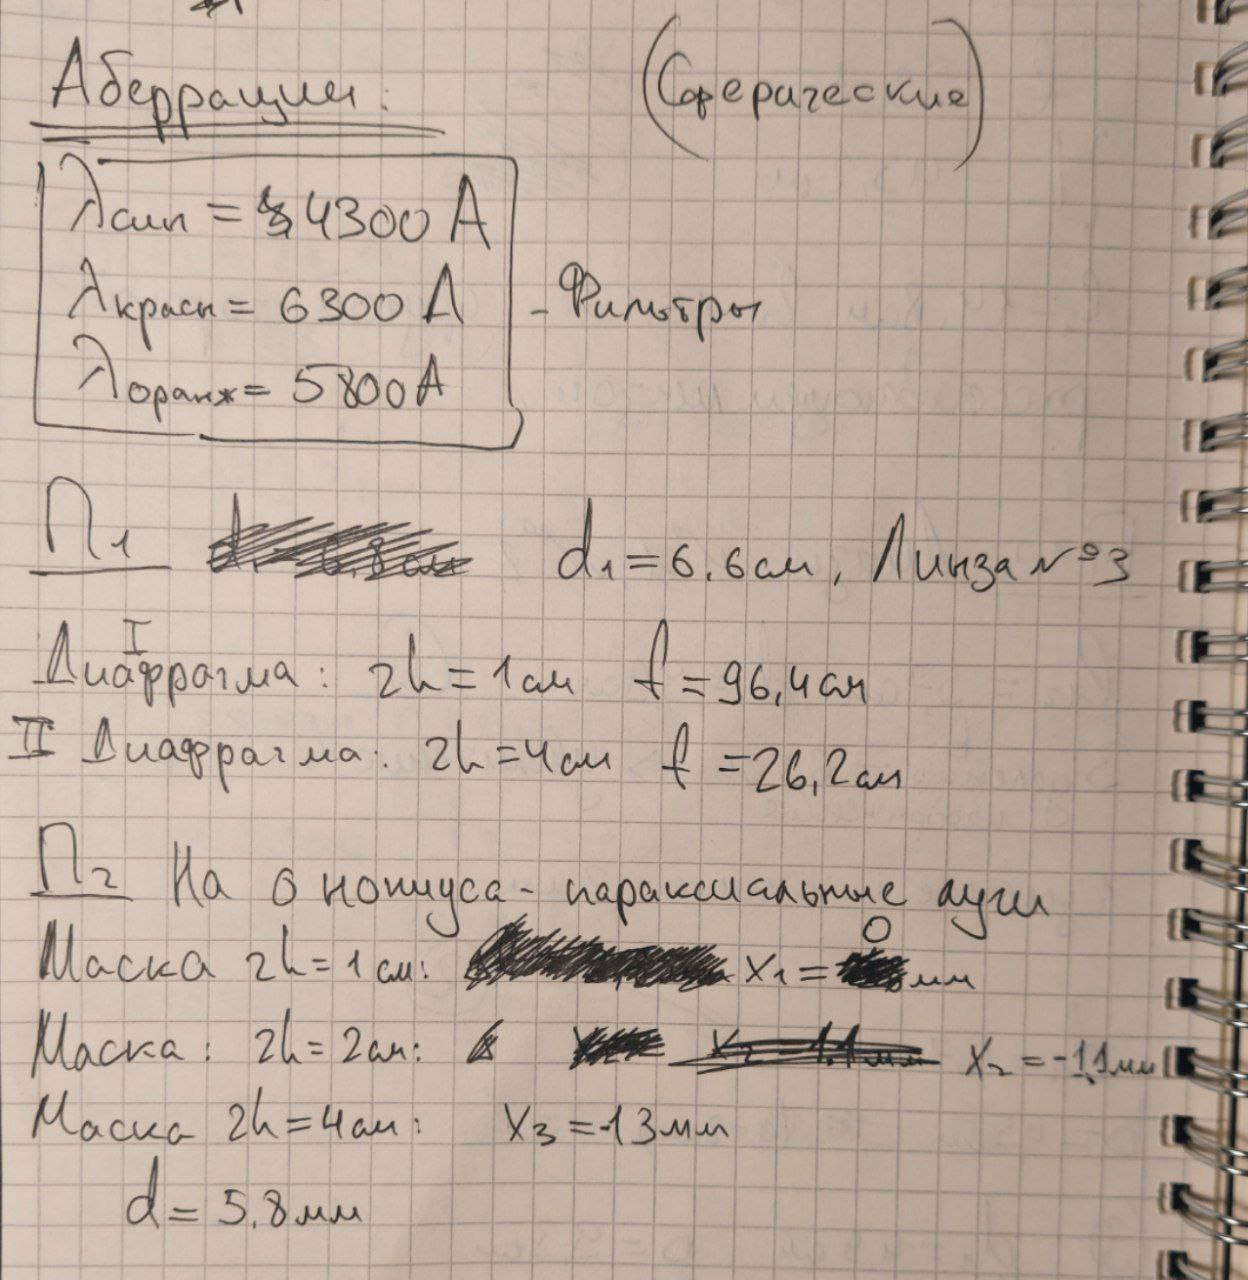
\includegraphics[width=0.3\textwidth]{../Изображения/6.jpg}
	\caption{Глаз зелёный верхний квадрат и оранжевый правый видел как прозрачные.}
\end{figure}

8. В работе было определено направление вращения эллиптически поляризованной волны -- правая поляризация.
	
	\section*{Обсуждение результатов и выводы}

В работе наблюдались кольца Ньютона. 

Был определён радиус кривизны линзы $R = 25,8 \pm 0,1 \mm$.

По наблюдению биений была определена разность длин волн желто-оранжевой и зелёной спектральных линий $\Delta \lambda = 32,1 \nm$.
Табличное значение длины волны жёлто-оранжевой спектральной линии $\lambda_1 = 578,2 \nm$. \\
Табличное значение длины волны зелёной спектральной линии $\lambda_2 = 546,1 \nm$. \\
Табличная разность длин волн $\Delta \lambda = 32,1 \nm$.
	
\end{document}